\documentclass{beamer}
\usetheme{Boadilla}
\usepackage{graphicx}
%\usepackage{comment}
\title{JAVA LAB}
\author{3rd chapter}
\date{\today}
\institute[SCIS, UOH] % Your institution as it will appear on the bottom of every slide, may be shorthand to save space
{
    \begin{figure}[H]
        \centering
        
\includegraphics[width=2cm, height=2cm]{university_logo.png}
    \end{figure}
    School of Computer and Information Sciences \\
    University of Hyderabad \\ % Your institution for the title page
\medskip
}
\begin{document}
\begin{frame}
    \titlepage
\end{frame}
\begin{frame}
    \tableofcontents
\end{frame}
\section{Inheritance}
\begin{frame}
    \frametitle{what is Inheritance?}
    It is mechanism in java in which one class is allow to inherit features of another class. The class
     which inherits features is known as subclass or child class. The other class, which is inherited is known as super class or parent class.
    \begin{figure}[H]
    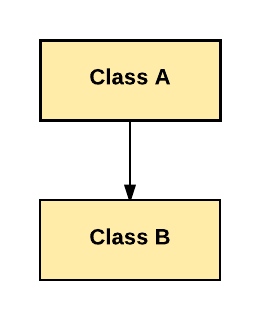
\includegraphics[scale=0.5]{images/single_inheritance.png}
    \end{figure}
\end{frame}
\begin{frame}
    \frametitle{Types of inheritance}
    \begin{enumerate}
        \item Single inheritance
        \item Multilevel inheritance
        \item Hierarchical inheritance
        \item multiple inheritance
    \end{enumerate}
    \begin{figure}[H]
        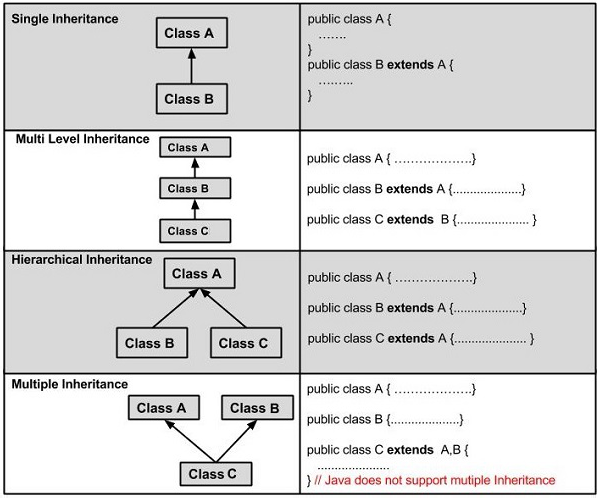
\includegraphics[scale=0.4]{images/types_of_inheritance.png}
    \end{figure}
\end{frame}
\section{method Overriding}
\begin{frame}
    \frametitle{method overriding}
    Overriding is a feature that allows a subclass or child class to provide a specific implementation of a method that is already provided by one of its super-classes or parent classes.\\ 
    textbf{example:}\\
        Class1:add()\\
        Class1 extends Class2(class2 inherits features from class1)\\
        Class2:add()\\
        it is possible in java\\
    Here is example program \href{inheritance_methodOveriding.java}{\color{green}{inheritance and methodOveriding}}
\end{frame}
\section{Overriding object class methods}
\begin{frame}
    \frametitle{Overriding object class methods}
    There is super class of all the classes we write, that is Object class. When we create a class that will be created as child class to object class. We can Override some methods in Object class.\\
    \textbf{methods in Object class:}\\
    \begin{enumerate}
        \item  protected Object clone() throws CloneNotSupportedException 
        \item public boolean equals(Object obj)
        \item protected void finalize() throws Throwable 
        \item public final Class getClass() --- cannot override 
        \item public int hashCode() 
        \item public String toString() 
        \item public final void notify() 
        \item public final void notifyAll() 
        \item public final void wait() 
        \item public final void wait(long timeout) 
        \item public final void wait(long timeout, int nanos)
    \end{enumerate}
    Here is the example of \href{Override_object.java}{\color{green}{Overriding Object class methods}} 
\end{frame}
\begin{frame}
    \frametitle{Polymorphism}
    Polymorphism is the ability of an object to take on many forms.\\

    Here is the example of \href{polymorphism.java}{\color{green}{Polymorphism}}
\end{frame}
\section{Abstract class}
\begin{frame}
    \frametitle{Abstract class}
    Abstract class is incomplete class in which atleast one method implementation is not there, if it is there also it will treated as incomplete class as we declare it as a abstract class.\\
    We cannot create an object to abstract class. In order to access members of abstract class, it must be inherited and abstract methods need to be implemented.\\
    we can create object for subclass.\\
    \textbf{Syntax:}\\
    abstract class Classname 
\end{frame}
\begin{frame}
    \frametitle{example of abstract class}
    \begin{figure}[H]
        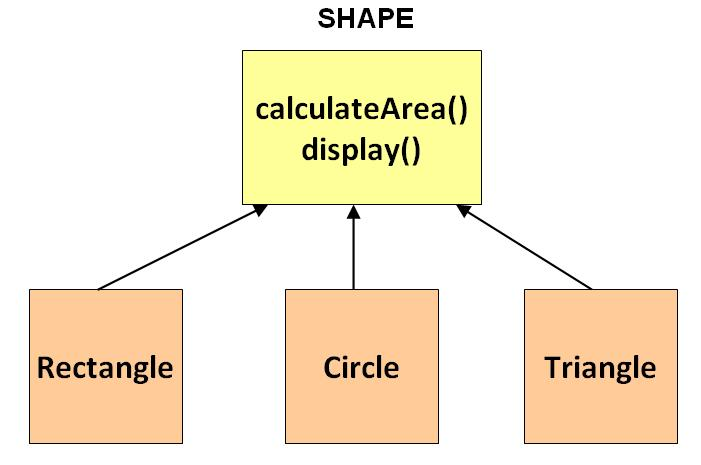
\includegraphics[scale=0.3]{images/java-abstract-classes.jpg}
    \end{figure}
    Shape class is abstract class.\\ 
    Here is the implementation of above example \href{abstract_class.java}{\color{green}{area of shape}} 
\end{frame}
\section{interface}
\begin{frame}
    \frametitle{interfaces}.
    The interface in Java is a mechanism to achieve abstraction.There can be only abstract methods in the Java interface, not method body. It is used to achieve abstraction. By using interfaces multiple inheritance is partially supported.\\
    \textbf{syntax:}\\
    interface Interfacename\\
    while inherited -- class Classname implements interfacename \\
    Here is the example \href{interface_example.java}{\color{green}{interface}}
\end{frame}
\section{garbage collector}
\begin{frame}
    \frametitle{garbage collector}
    In c, programmer is responsible for creating and destruction of objects.\\
    But in java the programmer need not to care for all those objects which are no longer in use. Garbage collector destroys these objects. \\
    It is deamon thread which is running in background always.\\
    Two ways of implementing garbage collector.\\
    \begin{enumerate}
        \item By using System.gc():
        \item By using Runtime.getRuntime().gc(); 
    \end{enumerate}
    Here is the example program of \href{garbage.java}{\color{green}{garbage collector}}.
\end{frame}
\end{document}